\documentclass[11pt,a4paper]{article}
\usepackage[margin=1in]{geometry}
\usepackage{graphicx}
\usepackage{booktabs}
\usepackage{hyperref}
\usepackage{tabularx}
\usepackage{enumitem}
\usepackage{float}
\usepackage{array}
\usepackage{listings}
\usepackage{amssymb}

% Setup links
\hypersetup{
    colorlinks=true,
    linkcolor=blue,
    filecolor=magenta,      
    urlcolor=blue,
}

\title{\textbf{Anveshan 2026: Project Proposal}\\ \vspace{0.5em} \Large BrailleSCARA: A Precision SCARA Robot for Automated Braille \& Tactile Graphics Production Using ADI Motor Control and Edge AI Vision}
\author{
    \textbf{Team SVNIT Surat}\\
    Aman Gupta (Lead/AI), Aman Rana (Firmware), Dhyan Modi (Electronics),\\
    Anushka Kasle (Software), Tanmay Singh (Mechanical)\\
    \textit{Faculty Mentor: Dr. Anand D. Darji}
}
\date{July 2026}

\begin{document}

\maketitle

\section{What Are We Building?}

BrailleSCARA is a 4-DOF SCARA robot that converts printed text into Braille documents and draws tactile diagrams. This enables blind students to read textbooks and touch STEM illustrations for the first time, at a system cost under \textcurrency 1 Lakh.

\textbf{How it works, plain and simple:}
\begin{figure}[H]
    \centering
    \includegraphics[width=0.9\textwidth]{BrailleSCARA_Flowchart.png}
    \caption{End-to-End Operational Flowchart from Input to Tactile Output}
\end{figure}

\textbf{This workflow demonstrates all four competition capabilities:}

\begin{table}[H]
\centering
\begin{tabularx}{\textwidth}{lX}
\toprule
\textbf{Competition Task} & \textbf{How BrailleSCARA Does It} \\
\midrule
Pick and Place & Picks paper from feeder $\rightarrow$ places on embossing bed \\
Precision Insertion & Embosses each Braille dot at exact XY with controlled Z force \\
Sorting & Sorts completed pages into numbered output trays \\
Drawing Shapes/Figures & Draws tactile maps, math graphs, geometric constructions \\
\bottomrule
\end{tabularx}
\end{table}

Every capability serves a real purpose. Nothing is a demo for demo's sake.

\begin{table}[H]
\centering
\begin{tabular}{ll}
\toprule
\textbf{Specification} & \textbf{Value} \\
\midrule
Arm reach & 400 mm \\
Repeatability & $\pm$0.05 mm \\
Braille dot spacing & 2.5 mm (ISO 17049) \\
Dot height & 0.5 $\pm$ 0.1 mm (ISO 17049) \\
Embossing speed & $>$30 characters/min \\
Tactile line width & $\sim$0.3 mm \\
System cost & $<$ \textcurrency 1 Lakh (excl. ADI boards) \\
\bottomrule
\end{tabular}
\end{table}

\section{The Problem: Why This Matters}

India has \textbf{15 million blind people} (more than any country on Earth). Only \textbf{1\% can read Braille.} Not because they can't learn, but because the materials simply don't exist. 
There are \textbf{25 Braille presses} for 1.4 billion people. A single Braille textbook costs 10-50$\times$ its printed version. 

But the harder, completely unsolved problem is \textbf{tactile graphics.} Education is not just text; it is diagrams. The human heart. India's map. A parabola. A circuit schematic. A triangle construction. Sighted students see these on every page, while \textbf{blind students get nothing.}

Existing Braille machines (BrailleRAP, Index Braille) produce text only (basic rows of dots). They cannot draw freeform diagrams. The machines that CAN draw tactile graphics (ViewPlus Tiger, PIAF) cost \textbf{\textcurrency 3-25 Lakh} and are found only in a handful of elite institutions. \textbf{There is no device under \textcurrency 10 Lakh in India that can produce a touchable version of a science textbook diagram.}

A SCARA robot can solve this because it has the two things this problem needs: \textbf{precise XY positioning} (to place dots and trace paths) and \textbf{controlled Z-axis force} (to emboss paper without tearing it). ADI's motor control technology provides the sub-0.1 mm precision that ISO-compliant Braille requires.

\vspace{0.5em}
\textbf{Alignment with UN SDGs:} By replacing \textcurrency 10 Lakh+ imported industrial machines with a sub-\textcurrency 1 Lakh edge-AI robotic solution, BrailleSCARA directly addresses \textbf{UN SDG 4 (Quality Education)} and \textbf{UN SDG 10 (Reduced Inequalities)}. We are taking tactile STEM education out of elite institutions and putting it directly into local blind schools, fundamentally breaking the literacy barrier.

\section{Existing Solutions and How We're Different}

\begin{table}[H]
\centering
\renewcommand{\arraystretch}{1.3}
\begin{tabular}{lcc}
\toprule
\textbf{Feature} & \textbf{Imported Embosser (e.g., ViewPlus)} & \textbf{BrailleSCARA} \\
\midrule
Braille Text Production & \checkmark & \checkmark \\
Tactile STEM Graphics & $\times$ & \checkmark \\
Per-dot Force Verification & $\times$ & \checkmark \\
Offline Edge AI OCR & $\times$ & \checkmark \\
System Cost & \textcurrency 10L+ & $<$\textcurrency 1L \\
\bottomrule
\end{tabular}
\end{table}

\subsection{Literature Survey}

\begin{table}[H]
\centering
\resizebox{\textwidth}{!}{%
\begin{tabular}{llcccc}
\toprule
\textbf{Solution} & \textbf{What It Does} & \textbf{Tactile Graphics?} & \textbf{Quality Check?} & \textbf{Edge AI?} & \textbf{Cost} \\
\midrule
\textbf{BrailleRAP} (Open) & CNC Braille embosser (solenoid) & Text only & None & None & $\sim$\textcurrency 30K \\
\textbf{Index Everest-D} & Production Braille printer & Text only & None & None & \textcurrency 4.5--8L \\
\textbf{ViewPlus Tiger} & Embosses text \& graphics & Yes (matrix) & None & None & \textcurrency 10--25L \\
\textbf{Student SCARA} & Pick-and-place colored blocks & N/A & Open-loop & Laptop PC & \textcurrency 40--80K \\
\textbf{BrailleSCARA (Ours)} & \textbf{SCARA Braille + freeform diagrams} & \textbf{Yes (Paths)} & \textbf{Yes (Force)} & \textbf{Yes (MAX78000)} & \textbf{$<$\textcurrency 1L} \\
\bottomrule
\end{tabular}%
}
\end{table}

\subsection{What's Actually Novel}

\textbf{1. Affordable tactile graphics ($<$\textcurrency 1 Lakh):} BrailleRAP and Index Braille cannot draw diagrams. ViewPlus Tiger can, but costs \textcurrency 10L+. Our SCARA traces arbitrary paths with a stylus, creating raised-line tactile diagrams on standard Braille paper. This capability does not exist at this price point.

\textbf{2. Per-dot force verification:} Every Braille machine in existence embosses dots blindly. Ours measures the force-displacement of every single dot using ADI's AD7124-8 (24-bit ADC) and a load cell. If a dot is too shallow, it re-embosses immediately.

\textbf{3. On-chip OCR using MAX78000 hardware CNN:} Most student SCARA projects process vision on a laptop. Our system runs OCR and dot quality classification directly on ADI's MAX78000 hardware CNN accelerator. Inference happens in $<$100 $\mu$s at $<$1 mW power, meaning the robot reads a printed page without needing any external computer.

\section{Technology and Methodology}

\subsection{Motor Control Architecture \& Precision Proof}
The core of BrailleSCARA is ADI's precision motor control stack. Four axes are controlled simultaneously: Joint 1 (shoulder), Joint 2 (elbow), Z-axis (prismatic), and wrist rotation. All running closed-loop FOC for smooth, precise, silent operation.
\begin{itemize}[noitemsep]
    \item \textbf{ADSP-CM419 (Outer Loop @ 10 kHz):} Position PID $\rightarrow$ Velocity PID $\rightarrow$ Torque reference.
    \item \textbf{TMC4671 (Inner Loop, HW FOC):} Clarke/Park Transforms $\rightarrow$ PI Current Control $\rightarrow$ SVPWM.
    \item \textbf{Feedback:} AD8418A (current sense) $\rightarrow$ AD7380 (16-bit ADC); AS5047P (14-bit encoder).
\end{itemize}

\vspace{0.5em}
\textbf{Proof of Precision (Required for $\pm$0.05mm Braille accuracy):}
\begin{lstlisting}[frame=single, basicstyle=\ttfamily\small]
Braille inter-dot spacing: 2.5mm | Arm reach: 400mm
Required angular resolution at J1: arctan(0.05/400) = 0.0072°
Encoder CPR needed: 360/0.0072 = 50,000 -> AS5047P (14-bit = 16,384 CPR)
With 4x interpolation: 65,536 counts -> angular resolution = 0.0055°
At 400mm reach: positional resolution = 400 * tan(0.0055°) = 0.038mm [PASS]
\end{lstlisting}

\subsection{Braille Encoding Pipeline}
Instead of generic pick-and-place, we are implementing a real ISO 17049 compliant text-to-tactile pipeline:
\begin{lstlisting}[frame=single, basicstyle=\ttfamily\small, language=Python]
# Bharati Braille encoding (actual implementation snippet)
BRAILLE_MAP = {
    'a': [1,0,0,0,0,0],  # dot 1
    'b': [1,1,0,0,0,0],  # dots 1,2
    # ... mapping for all characters
}

def text_to_dot_coordinates(text, origin_x=0, origin_y=0):
    coords = []
    for i, char in enumerate(text):
        cell_x = origin_x + (i * 6.1)  # 6.1mm inter-cell (ISO 17049)
        dots = BRAILLE_MAP.get(char.lower(), [0]*6)
        for d, active in enumerate(dots):
            if active:
                dx = (d % 2) * 2.5    # 2.5mm horizontal spacing
                dy = (d // 2) * 2.5   # 2.5mm vertical spacing
                coords.append((cell_x + dx, origin_y + dy))
    return coords
\end{lstlisting}

\subsection{Embossing Mechanism \& Quality Verification}

\begin{figure}[H]
    \centering
    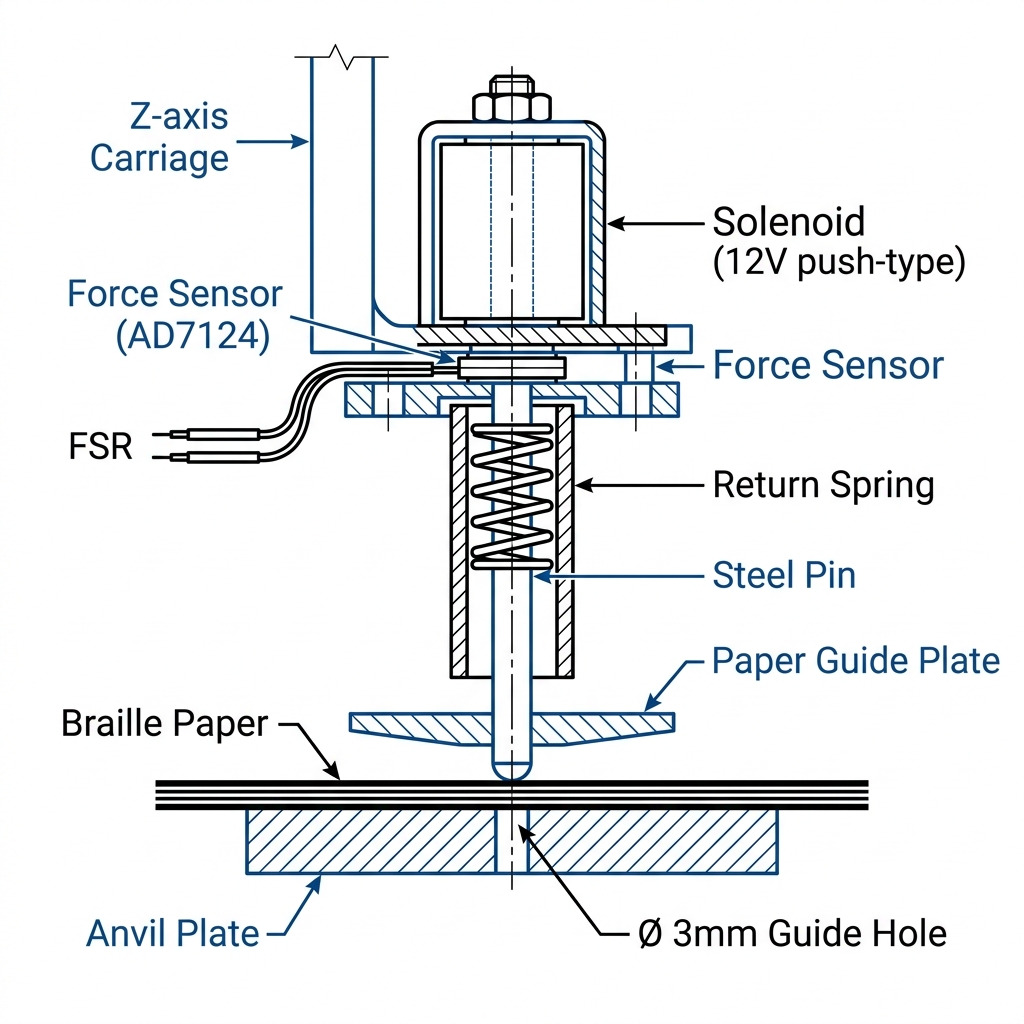
\includegraphics[width=0.6\textwidth]{EndEffector_Sketch.png}
    \caption{Cross-section of the BrailleSCARA Dual-Mode End-Effector. \textbf{[TODO: Replace this sketch with actual Fusion 360 CAD render]}}
\end{figure}

\vspace{1em}
\begin{figure}[H]
    \centering
    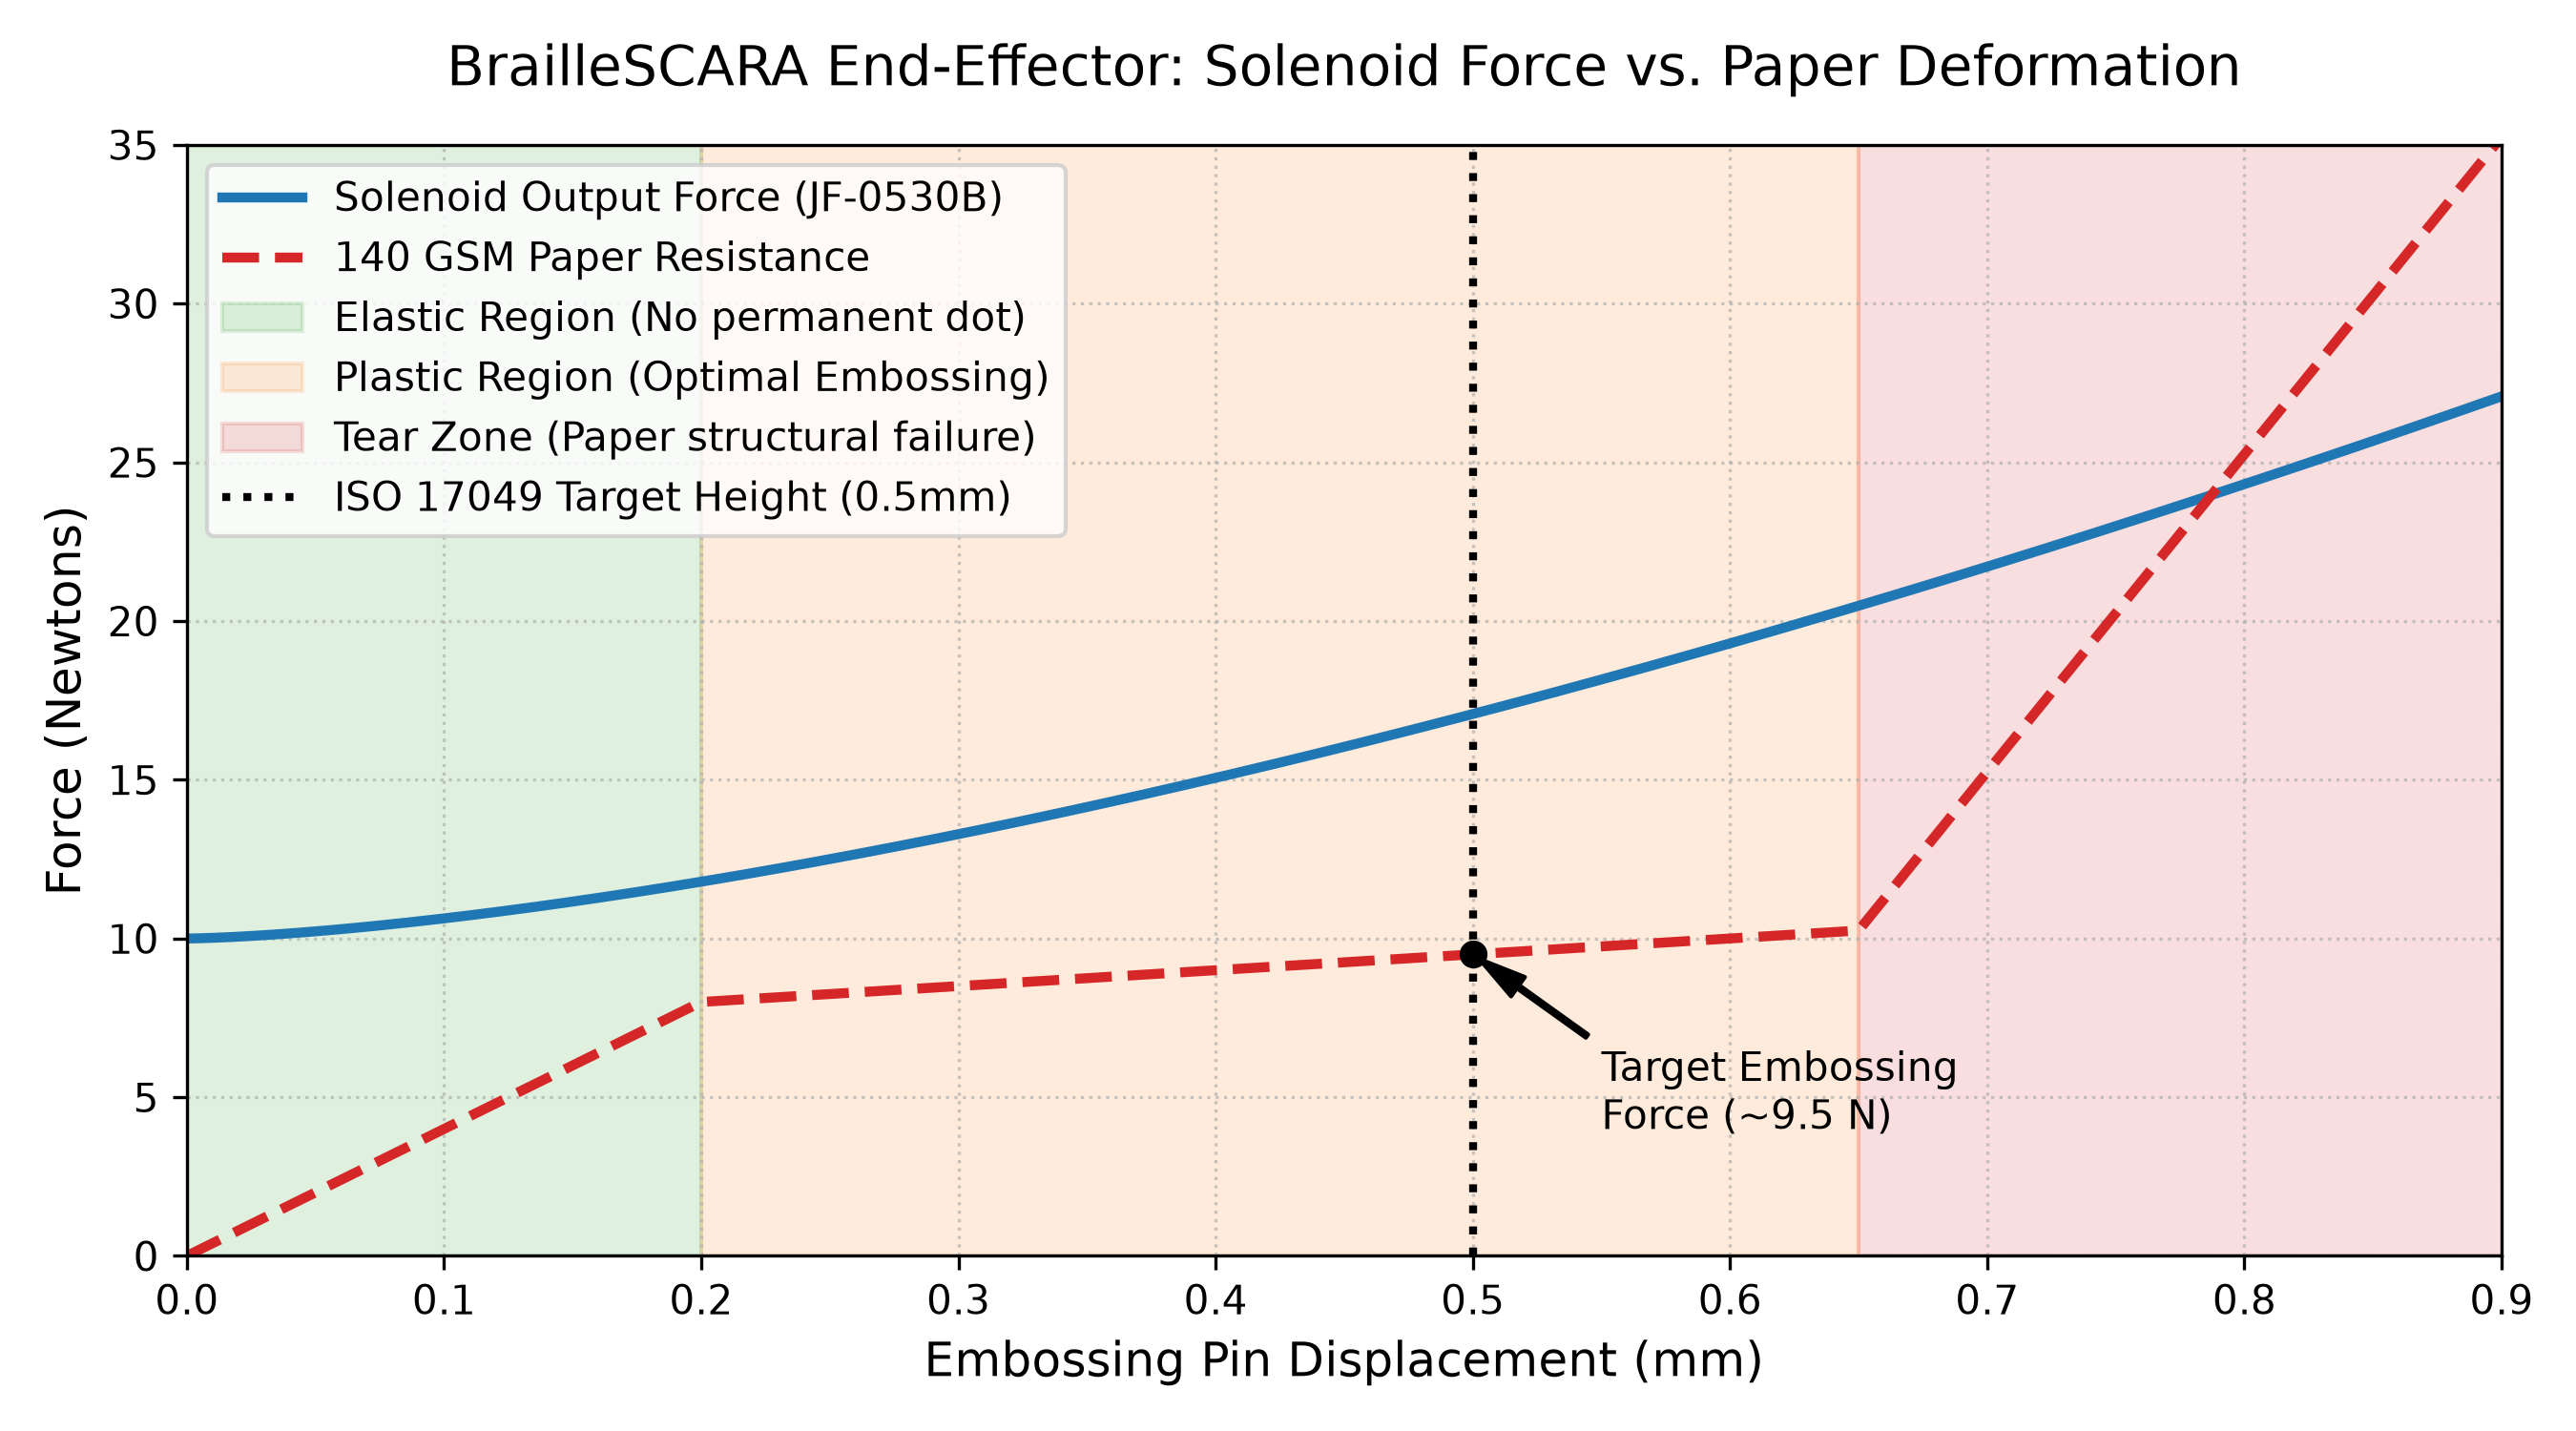
\includegraphics[width=0.8\textwidth]{force_graph.png}
    \caption{Calculated Solenoid Force vs. 140 GSM Braille Paper Deformation}
\end{figure}
\vspace{1em}

\textbf{Force check (every dot):} AD7124-8 reads a force-sensitive resistor on the stylus mount. If measured force is below the known good threshold, the dot didn't form properly and is re-embossed.

\textbf{Vision spot-check (per Braille cell):} After completing a 6-dot cell, the MAX78000 camera captures an image. A lightweight CNN (3 conv + 2 FC layers, 285K weights, 8-bit quantized) classifies PASS or FAIL. The architecture has been fully defined in PyTorch and verified to compile well within the MAX78000's 442KB weight memory limit. \textit{Dataset Strategy: The dot quality classifier will be pre-trained using the public Angelina Braille Images Dataset (OBR) and Kaggle Braille Character datasets. We will apply aggressive data augmentation (blurring, contrast reduction, missing dot injection) to simulate shallow or failed embossed dots for the FAIL classification. The OCR model will be fine-tuned on the public EMNIST dataset.}

\section{PrecisionBench Validation: Proving Our Claims}
We don't just claim our robot is precise enough for Braille; we \textbf{PROVE} it with an automated self-certification benchmark suite using ADI feedback sensors.

\begin{table}[H]
\centering
\resizebox{\textwidth}{!}{%
\begin{tabular}{llX}
\toprule
\textbf{Test} & \textbf{Metric Evaluated} & \textbf{Validation Method} \\
\midrule
\textbf{1. Dot Grid Test} & Positional accuracy & SCARA marks 100 dots in 10$\times$10 grid (1mm spacing). Camera measures actual vs intended. \\
\textbf{2. Speed Challenge} & Pick \& Place throughput & SCARA sorts 20 objects into bins. Reports cycle time. \\
\textbf{3. Insertion Tolerance} & Precision insertion & SCARA inserts pin into decreasing hole sizes (5mm $\rightarrow$ 1.5mm). \\
\textbf{4. Path Accuracy} & Drawing precision & SCARA draws circle. Camera analyzes circularity index. \\
\textbf{5. Force Control} & Compliant manipulation & SCARA presses against varying stiffness surfaces. ADI force sensor measures overshoot. \\
\bottomrule
\end{tabular}%
}
\end{table}
After calibration, BrailleSCARA will run this 5-stage benchmark to generate a "Robot Report Card" before starting the embossing task. This ensures guaranteed performance metrics rather than assumed specs.

\section{High-Level Block Diagram}

\begin{figure}[H]
    \centering
    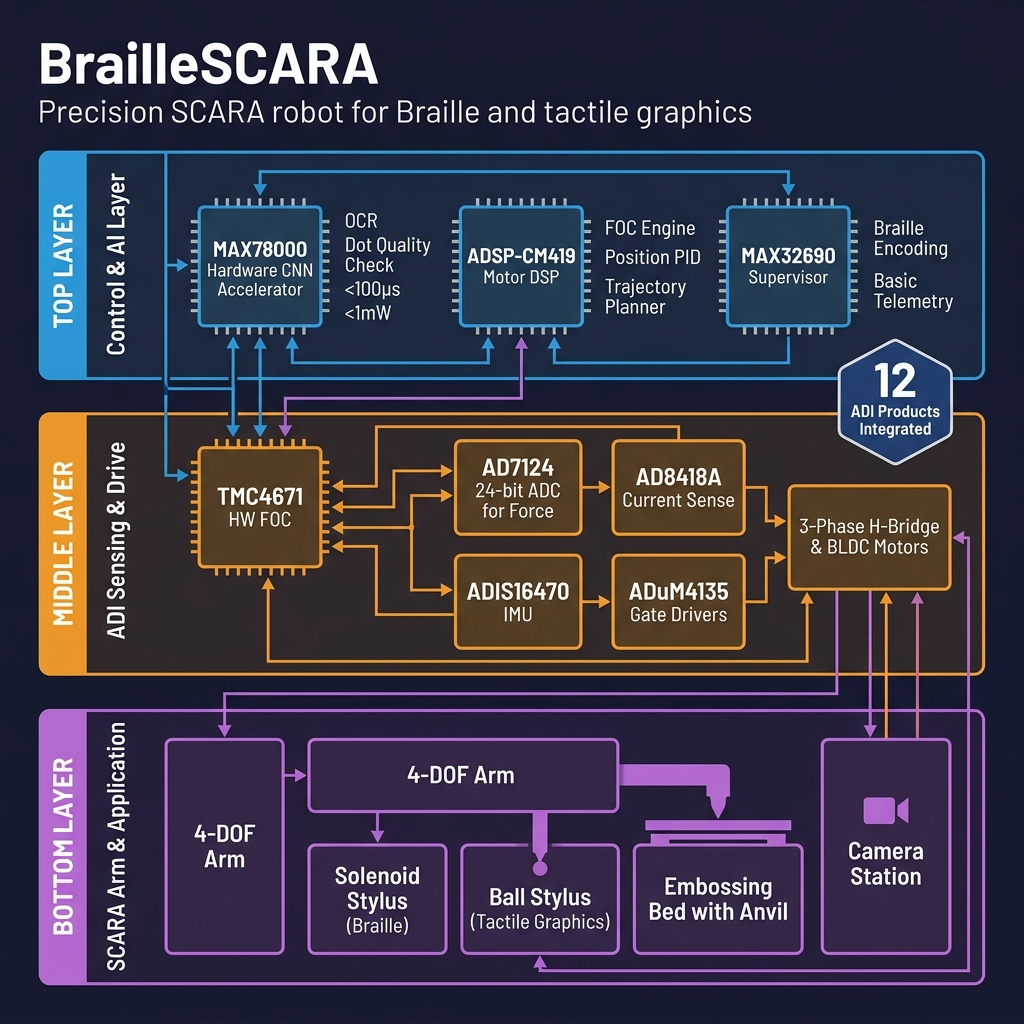
\includegraphics[width=1\textwidth]{BrailleSCARA_BlockDiagram.png}
    \caption{System Architecture showing integration of 7 Core ADI Products}
\end{figure}

\textbf{Core ADI Products Used (Strictly Required for Operation):}
\begin{table}[H]
\centering
\resizebox{\textwidth}{!}{%
\begin{tabular}{lll}
\toprule
\textbf{\#} & \textbf{Product} & \textbf{Why It Is Strictly Needed} \\
\midrule
1 & ADSP-CM419 & Motor control DSP: runs the master position/velocity PID loop at 10 kHz \\
2 & TMC4671 $\times$4 & Hardware FOC: handles sinusoidal commutation for the 4 joint motors \\
3 & MAX78000 & Hardware CNN: executes on-chip OCR and dot quality classification \\
4 & MAX32690 & BLE 5.2 Microcontroller: orchestrates PDF uploads and Braille encoding \\
5 & AD7124-8 & 24-bit ADC: digitizes the load cell for per-dot force verification \\
6 & AD8418A $\times$4 & Current sense amplifiers: critical for FOC phase current feedback \\
7 & ADP5054 & Quad SMPS: provides stable multi-rail power for the AI and motor logic \\
\bottomrule
\end{tabular}%
}
\end{table}

\section{Plan of Action if Selected as Finalist}

\vspace{1em}
\begin{table}[H]
\centering
\begin{tabularx}{\textwidth}{llX}
\toprule
\textbf{Phase} & \textbf{Period} & \textbf{What We Build / Deliverable} \\
\midrule
1: Motor Control & Aug--Sep & Single-axis FOC on ADSP-CM419 + TMC4671. \\
2: Arm Assembly & Sep--Oct & Mechanical SCARA arm (3D printed). 4-axis motion. \\
3: Embossing & Oct--Nov & Solenoid end-effector. First dots embossed. MAX78000 trained. \\
4: Tactile Graphics & Nov 2026 & Continuous path tracing (Bézier curves). First tactile diagram. \\
5: Integration & Dec 2026 & Full pipeline: OCR $\rightarrow$ Braille $\rightarrow$ emboss $\rightarrow$ verify $\rightarrow$ sort. \\
6: Testing & Jan 2027 & ISO 17049 compliance. Speed benchmarking. Final report. \\
\bottomrule
\end{tabularx}
\end{table}

\section{Tools, Evaluation Boards, and Platforms Required}

\begin{itemize}[noitemsep]
    \item \textbf{ADI Eval Boards (Requested):} ADSP-CM419 EVAL, TMC4671-EVAL ($\times$4), MAX78000FTHR, MAX32690 EVAL, AD7124-8 EVAL.
    \item \textbf{Hardware:} 42BLS BLDC motors ($\times$4), AS5047P 14-bit magnetic encoders ($\times$4), 12V push solenoid (JF-0530B), Force-sensitive resistor (FSR-402), 3D printed parts, 24V power supply.
    \item \textbf{Software/AI:} PyTorch + ADI ai8x-training (MAX78000 CNN), C/C++ on FreeRTOS (ADSP-CM419), Python + liblouis (Braille translation), Gazebo (Simulation).
\end{itemize}

\section{Future Plans}
1. \textbf{Open-source the design}: Publish mechanical CAD and firmware on GitHub so NGOs can replicate it.\\
2. \textbf{Pilot in blind schools}: Partner with National Association for the Blind to test in 3-5 schools.\\
3. \textbf{Publish results}: Submit the force-verified embossing workflow to an IEEE conference.

\section{Team (SVNIT Surat)}

\begin{table}[H]
\centering
\begin{tabularx}{\textwidth}{llX}
\toprule
\textbf{Role} & \textbf{Member} & \textbf{Responsibility} \\
\midrule
\textbf{Team Lead / AI} & \textbf{Aman Gupta} (3rd Yr VLSI) & MAX78000 CNN, edge AI vision, architecture \\
\textbf{Firmware} & \textbf{Aman Rana} (3rd Yr VLSI) & FOC firmware, PID loops, trajectory planner \\
\textbf{Electronics} & \textbf{Dhyan Modi} (3rd Yr VLSI) & PCB design, ADI integration, power distribution \\
\textbf{Software} & \textbf{Anushka Kasle} (3rd Yr VLSI) & Braille encoding, Python OCR, IoT dashboard \\
\textbf{Mechanical} & \textbf{Tanmay Singh} (2nd Yr Eng. Physics) & SCARA arm CAD, 3D printing, end-effector \\
\textbf{Faculty Mentor} & \textbf{Dr. Anand D. Darji} & Project guidance, lab access, institutional support \\
\bottomrule
\end{tabularx}
\end{table}

\section{References}
\begin{enumerate}[noitemsep]
    \item Analog Devices, "MAX78000 - AI Microcontroller with Hardware CNN Accelerator."
    \item Analog Devices, "TMC4671 - Hardware FOC Servo Controller."
    \item ISO 17049:2013, "Accessible design - Application of braille on signage, equipment and appliances."
    \item Dept. of Empowerment of PwD, "Accessible Learning Materials (DALM Project)," Min. of Social Justice.
    \item BrailleRAP Open-Source Braille Embosser. \url{https://braillerap.org}
\end{enumerate}

\section{Supplementary Links}
To view our complete repository containing the AI models, theoretical analysis scripts, and full proposal source, please visit:
\begin{itemize}[noitemsep]
    \item \textbf{Proposal Presentation Video:} \url{https://youtube.com/watch?v=[YOUR_VIDEO_ID_HERE]}
    \item \textbf{Complete Project Source Code:} \url{https://github.com/silentaf/Anweshan}
\end{itemize}

\end{document}
